\documentclass[11pt,border=5pt]{standalone}
\usepackage{fontspec}
\setmainfont{cmunrm.otf}[BoldFont=cmunbx.otf,ItalicFont=cmunti.otf,BoldItalicFont=cmunbi.otf]
\usepackage{amsmath}
\usepackage{unicode-math}
\setmathfont{NewCMMath-Regular.otf}
\usepackage{tikz}
\usetikzlibrary{arrows.meta,patterns,angles,quotes}
\begin{document}
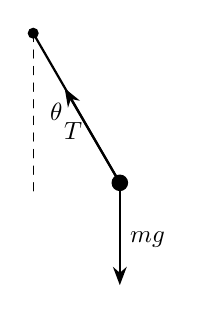
\begin{tikzpicture}[>=Stealth,font=\small,line cap=round,line join=round]
\draw[thick] (0,1.5) -- (1.1,-0.4);
\fill (0,1.5) circle (2pt);\fill (1.1,-.4) circle (3pt);
\draw[->,thick] (1.1,-0.4) -- (0.4,0.8) node[pos=0.55,left] {$T$};
\draw[->,thick] (1.1,-0.4) -- (1.1,-1.7) node[pos=0.55,right] {$mg$};
\draw[dashed] (0,1.5) -- (0,-0.6);
\node at (0.3,0.5) {$\theta$};

\end{tikzpicture}
\end{document}
